\subsection{Pseudocode}
\begin{aufgabe}
\TeX en Sie folgenden Pseudocode so exakt wie m\"oglich nach.\\

\noindent \underline{Ursprung:} \\
\noindent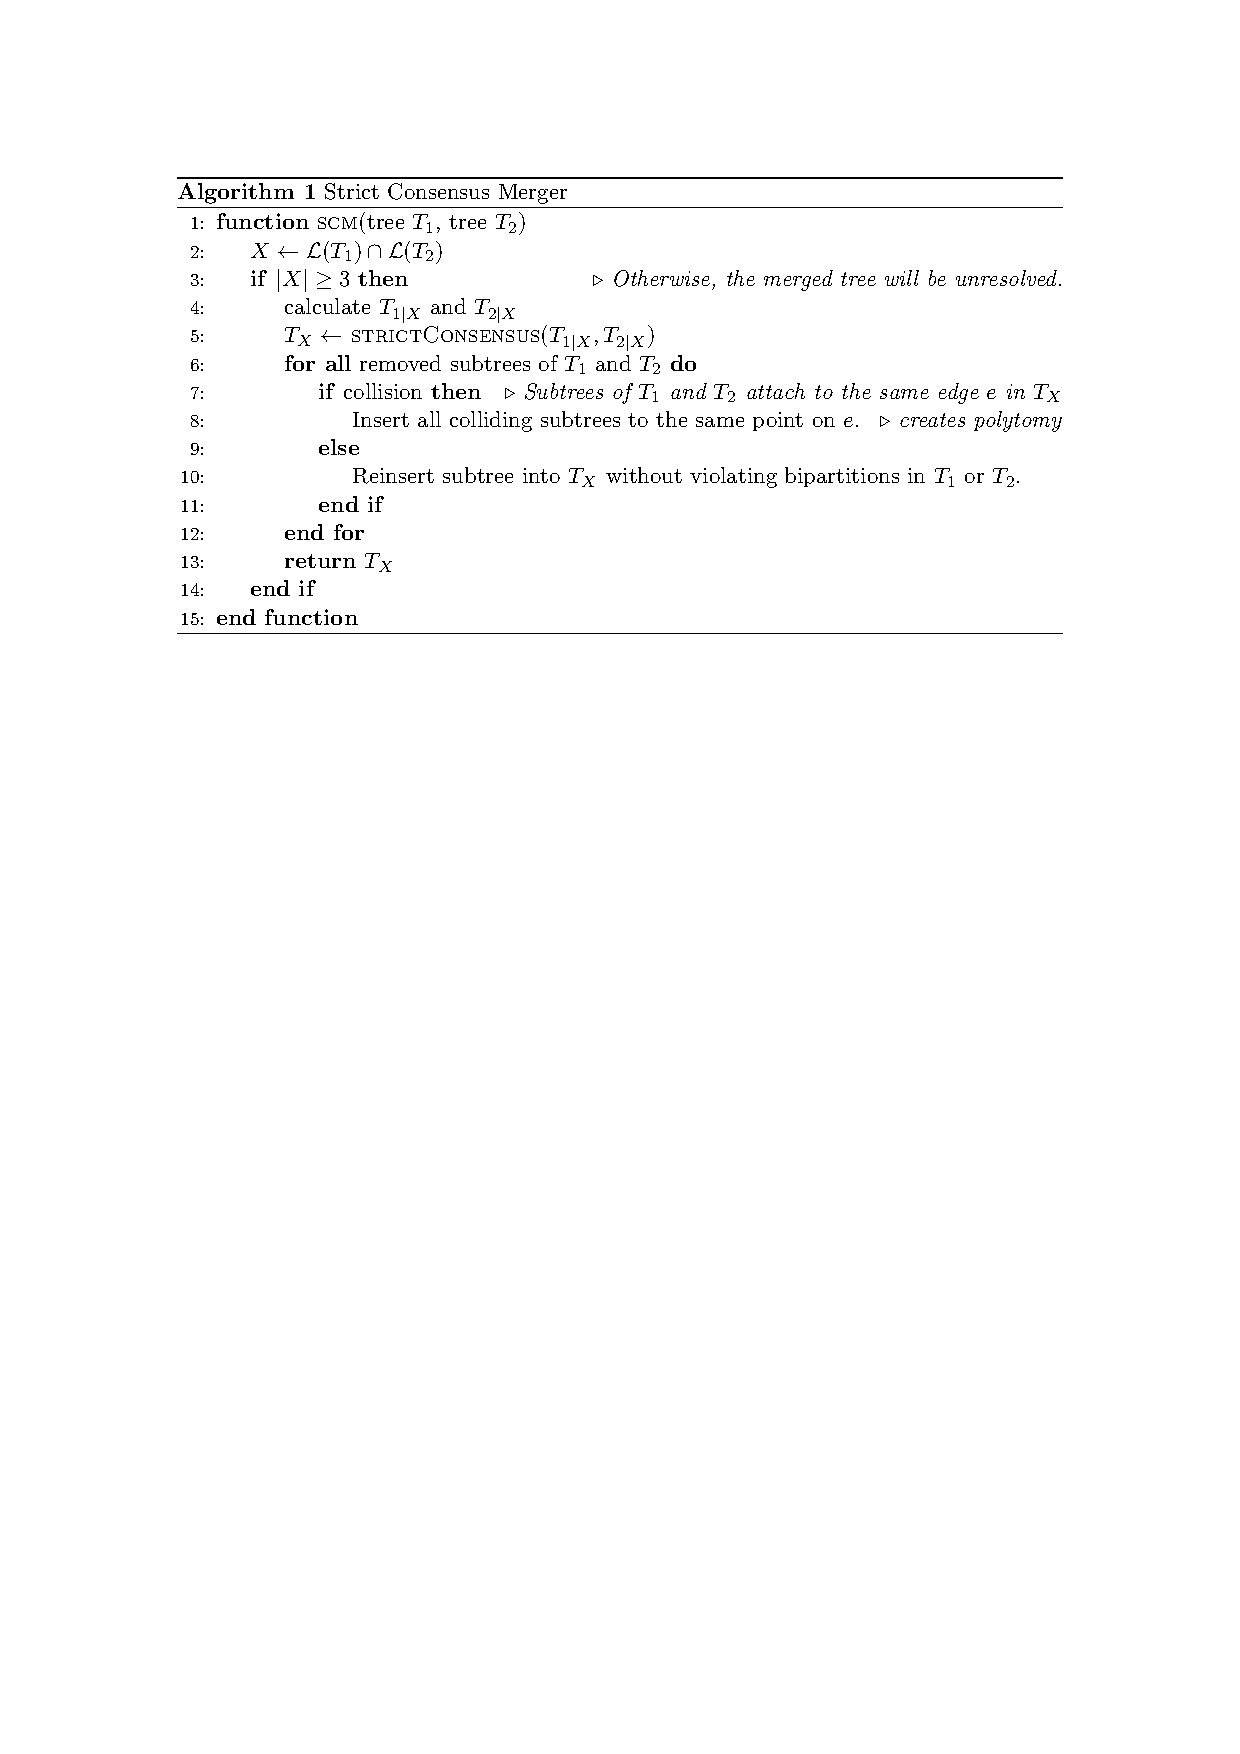
\includegraphics[width=\textwidth]{aufgabe36}	

\noindent \underline{nachge\TeX t:}\\
\begin{algorithm}
   \caption{Strict Consensus Merger}
    \begin{algorithmic}[1]
      \Function{scm}{tree $T_1$, tree $T_2$}
	\State $X \leftarrow \mathcal{L}(T_1) \cap \mathcal{L}(T_2)$
        \If {$|X| \geq 3$}	\Comment{\textit{Otherwise, the merged tree will be unresolved.}}
        \State calculate $T_{1|X}$ and $T_{2|X}$
        \State $T_X \leftarrow$ \Call{strictconsensus}{$T_{1|X},T_{2|X}$}
        \ForAll{removed subtrees of $T_1$ and $T_2$}
	  \If{collision}	\Comment{\textit{Subtrees of $T_1$ and $T_2$ attach to the same edge e in $T_X$}}
	    \State{Insert all colliding subtrees to the same point on $e$.}   \Comment{\textit{creates polytomy}}
	  \Else
	    \State{Reinsert subtree into $T_X$ without violating bipartitions in $T_1$ or $T_2$.}
	  \EndIf
	  \EndFor \\
	\ \  \  \ \ \ \ \ \ \Return{$T_X$}
	\EndIf
       \EndFunction
\end{algorithmic}
\end{algorithm}

\end{aufgabe}

\pagebreak
\subsection{Sourcecode}
\begin{aufgabe}\label{aufg:sourceCode}
\TeX en Sie den Quelltext aus \texttt{aufgabe\ref{aufg:sourceCode}.pdf} so exakt wie m\"oglich nach.(Quelltext: \texttt{AbstractSCMAlgorithm.java})\\ 
\end{aufgabe}

\lstset{ 
  backgroundcolor=\color{white},
  basicstyle=\footnotesize\ttfamily,
  breakatwhitespace=false,
  breaklines=true,
  captionpos=b,
  commentstyle=\color{mygreen},
  deletekeywords={...},
  escapeinside={\%*}{*)},
  extendedchars=true,
  frame=single,
  keepspaces=true,
  keywordstyle=\color{myred},
  language=Java,
  morekeywords={*,...},
  numbers=left,
  numbersep=5pt,
  numberstyle=\tiny\color{mygray},
  rulecolor=\color{white},
  showspaces=false,
  showstringspaces=false,
  showtabs=false,
  stepnumber=1,
  stringstyle=\color{mygray},
  tabsize=4,
  title=\lstname,
  emph={@Override},
  emphstyle={\color{mygold}}
}

\lstinputlisting[language=java]{src/AbstractSCMAlgorithm.java}